\documentclass{exam}
\usepackage[utf8]{inputenc}
\usepackage{color}
\usepackage{amsmath}
\usepackage[english]{babel}
\usepackage{comment}
\usepackage{graphicx}
\usepackage{wrapfig}
\usepackage{caption}
\usepackage{subcaption}
\usepackage[siunitx]{circuitikz}
\newcommand{\splitcell}[2][c]{%
  \begin{tabular}[c]{@{}c@{}}\strut#2\strut\end{tabular}%
}
\usepackage{natbib}
\usepackage{listings}
\usepackage{xparse}
\usepackage{hyperref}
\usepackage{float}
\usepackage{tcolorbox}

\NewDocumentCommand{\codeword}{v}{%
\texttt{\textcolor{blue}{#1}}%
}
\usepackage{pgfplots}
\pgfplotsset{compat = newest}
\usepackage{chngcntr}
\counterwithin{table}{section}
\counterwithin{figure}{section}

\usepackage{listings}
\usepackage{xcolor}

\definecolor{codegreen}{rgb}{0,0.6,0}
\definecolor{codegray}{rgb}{0.5,0.5,0.5}
\definecolor{codepurple}{rgb}{0.58,0,0.82}
\definecolor{backcolour}{rgb}{0.95,0.95,0.92}

\lstdefinestyle{mystyle}{
    backgroundcolor=\color{backcolour},   
    commentstyle=\color{codegreen},
    keywordstyle=\color{magenta},
    numberstyle=\tiny\color{codegray},
    stringstyle=\color{codepurple},
    basicstyle=\ttfamily\footnotesize,
    breakatwhitespace=false,         
    breaklines=true,                 
    captionpos=b,                    
    keepspaces=true,                 
    numbers=left,                    
    numbersep=5pt,                  
    showspaces=false,                
    showstringspaces=false,
    showtabs=false,                  
    tabsize=2
}

\lstset{style=mystyle}

\begin{document}

\newcommand{\Exjobbsnummer}[1]{
	\begin{tikzpicture}[overlay, remember picture]
		\path (current page.north east) ++(-1,-1) node[below left] {{\small #1}};
	\end{tikzpicture}
}

\newcommand{\Examensjobbspoang}[1]{
	\begin{tikzpicture}[overlay, remember picture]
		\path (current page.north east) ++(-1,-1.5) node[below left] {{\normalsize \scshape Examensarbete #1 HP}};
	\end{tikzpicture}
}

\newcommand{\datum}[1]{
	\begin{tikzpicture}[overlay, remember picture]
		\path (current page.north east) ++(-1,-2.0) node[below left] {{\normalsize #1}};
	\end{tikzpicture}}

\newcommand{\storlitentitel}[2]{
\center
\rule[0.2cm]{13cm}{0.1cm}
{ \huge \bfseries #1}\\[0.4cm] % Title of your document
{\Large \slshape #2}\\[0.4cm]
\rule[0.2cm]{13cm}{0.1cm}\\[3cm]

}

\newcommand{\Namn}[2]{
	\begin{minipage}{0.5\textwidth}
		\normalsize
		\centering
		#1 \textsc{#2}\\
	\end{minipage}\\
}

\newcommand{\LoggaSwe}{
	\textsc{\Huge Internet Performance \\[0.3cm] and Troubleshooting Lab}\\[0.7cm]
	
\includegraphics[scale=.06]{polito_logo_2021_blu.jpg}\\[1.5cm]
}

\newcommand{\LoggaEng}{
	\textsc{\Huge Uppsala University}\\[0.7cm]
	\includegraphics[scale=.1]{Uppsala_University_seal_svg.png}\\[0.5cm]
}

% -----------------------------------------------
%           HÄR BÖRJAR TITELSIDAN
%------------------------------------------------
\begin{titlepage}

	\center

	%-------------------------------------------------
	%	INFORMATION ATT FYLLA I
	%-------------------------------------------------
	\Exjobbsnummer{Academic Year 2023/2024}
	%\datum{2021/2022}

	\LoggaSwe
	% \LoggaEng - Byt till engelska

	\storlitentitel{\\Report IV}{Impact of RTT and Packet Loss}

	\Large Group 3\\
	\Namn{Brendon Mendicino}{(s317639)}
	\Namn{Alessandro Ciullo}{(s310023)}
	\Namn{Davide Colaiacomo}{(s313372)}

	\vfill

\end{titlepage}
\pagebreak

\section{Configuration}
Before conducting the experiment, we set up the client with the following configuration: first of all, we enabled the \verb|TCP_Diag| module with the command:
\begin{lstlisting}
    modprobe tcp_diag
\end{lstlisting}
Then, we enabled the \verb|tcp log tracing| by means of the following command in the \verb|/sys/kernel/debug/tracing| directory:
\begin{lstlisting}
    echo 1 > events/tcp/tcp_probe/enable
\end{lstlisting}
By using the \verb|systemctl| tool, we enabled the \verb|TCP Selective Acknowledgment|:
\begin{lstlisting}
    sysctl net.ipv4.tcp_sack=1
\end{lstlisting}
During the experiments, all the offloading capabilities of the \textbf{NIC} were disabled with the command:
\begin{lstlisting}
    ethtool -K ${INTF} rx off tx off sg off tso off gso off gro off
\end{lstlisting}
Finally, the channel speed was set to 10Mbps. All experiments were done with two PC connect with point-to-point Ethernet cable, and all the captures where performed using \texttt{iperf3}.

\section{\texttt{tcp\_diag}}
\verb|tcp_diag| is a kernel module used to monitor the internal values of the \textbf{TCP} algorithm, such as the value of the \texttt{Congestion Window} (\textbf{CWND}), the \texttt{Slow start Threshold} (\textbf{SSTRESH}), and other parameters. Unfortunately, this way of tracing the \textbf{TCP} state is not the most precise from the point of view of the packets sent; the reason is that all of these values are fetched when an \textbf{ACK} is received by the system and not when a packet is sent, thus causing some of them to be not precise, like the \texttt{Seq-No.} or the \texttt{packet length}. This is done in order to avoid overloading the system when it is sending the segments in loop; in fact, we can see that the majority of the segments have \texttt{payload length} equal to 0, signaling that there are no data being sent in that specific moment by the kernel. This way of reading the data is consistent with the fact that, in the \texttt{Linux kernel}, parameters such as \textbf{CWND} and \textbf{SSTRESH} are updated when an \textbf{ACK} is received; as a matter of fact, by looking at the implementation of the \texttt{slow-start} phase in the kernel, it is possible to see that the \textbf{CWND} is updated when the next packet is acknowledged:
\begin{lstlisting}[language=c]
__bpf_kfunc u32 tcp_slow_start(struct tcp_sock *tp, u32 acked)
{
	u32 cwnd = min(tcp_snd_cwnd(tp) + acked, tp->snd_ssthresh);

	acked -= cwnd - tcp_snd_cwnd(tp);
	tcp_snd_cwnd_set(tp, min(cwnd, tp->snd_cwnd_clamp));

	return acked;
}
\end{lstlisting}
It is also interesting to note that this piece of code is the source of the exponential growth of the \texttt{slow-start} phase.

\section{Delay vs. Loss}
All the algorithm we tested were based on either one of two premises: \textit{"Decrease the CWND based on the lost segments recorded"} vs \textit{"Decrease the CWND based on the delay of the ACK segments recorded"}, one of them though (\textbf{BBR}) is based on delay to adjust the \textbf{CWND}, but it doesn't quite fit how the others \textbf{TCP} CCAs are fair between each other.

\section{Reno}
\textbf{Reno} was among the first algorithms implemented for the \texttt{TCP Congestion Control}; the implementation consists of a simple \texttt{Additive Increase - Multiplicative Decrease}, which means that it will be very sensible to packet losses, especially with modern connections that, in some instances, might also reach speeds of 10Gb/s. The \textbf{Reno} implementation that is currently adopted in the \texttt{Linux kernel} is the \textbf{New Reno}, which is an improved version of the original one; more than one change has been made in \textbf{New Reno}, but the one we can observe from the graphs is the following: in \textbf{New Reno}, losses do not make the algorithm get back to the \texttt{Slow start} phase, they just halve the \textbf{CWND} and continue from there in \texttt{Congestion Avoidance} mode.

By observing image \ref{fig:cubic-vs-reno} (b) and image \ref{fig:reno_cwnd_comparison}, we can understand the differences that become more evident when different delays and different packet loss percentages are used. 
The first thing that catches our attention is the growth of the \textbf{CWND}, with 0\% or 0.01\% of packet loss, that reaches a size of \texttt{4500} (a limit set by the kernel) and then stops growing; furthermore, the \textbf{CWND} seems to grow linearly, instead of exponentially. This is caused by the channel speed, in the sense that a speed of 10Mbps with small \textbf{RTT} (10ms or 50ms) can be supported by the \texttt{Congestion Control} when the \textbf{CWND} size is about $ \frac{10Mbps * RTT}{8 * 1538}$; with a delay of 10ms, the needed size is around 10, so only 4 \texttt{round-trip} times (\textbf{RTT}) must pass for the channel to be saturated, making it hard for it to appear on the graph; we can only see a little trace of the classical exponential \texttt{Slow start} shape in the first part of image \ref{fig:reno_cwnd_comparison} with 200ms of delay. After that, even if the congestion window increases (as observable from the graph and the \texttt{Linux kernel} source code), the growth is limited by the channel's speed, and we know that if the growth is constant, the function is linear. The \texttt{0.01\% packet loss} graph acts in the same way as the \texttt{0\% packet loss} graph because, in the sample that has been taken, the loss never happened.

By continuing the analysis, we can observe how with packet loss percentage \> 0.01\%, the graphs are pretty different; after a first \texttt{slow start} phase, when a loss occurs, the \texttt{Congestion Control} passes to the \texttt|Congestion Avoidance| phase by setting the threshold to the last \textbf|CWND/2| and starting an additive increase of 1 \texttt{Maximum Segment Size} (\textbf{MSS}) for each \texttt{RTT}. Since the amount of loss is significant, the growth of the \textbf|CWND| is slower than the reduction caused by the loss and the congestion window inevitably reaches values close to zero.

Another curious phenomenon is the variation of the \texttt{Round-Trip Time} (\textbf{RTT}) across different loss percentages graphs; by observing figure \ref{fig:reno_rtt_comparison}, what is surprising to notice are the around two seconds \textbf|RTT| we get over an Ethernet cable when no loss or nearly no loss occur. This is caused by the enormous congestion window we discussed before; the kernel generates and send to the \textbf{NIC} all those packets until the \textbf{NIC}'s memory is full, creating a roughly 2 seconds long queue for every packet after a certain point. For packet losses > 0.01\%, the \textbf{RTT} has a big growth during the \texttt{slow start} phase, but as soon as losses occur, the \textbf|CWND| decreases drastically and no queue is created; the \verb|RTT| is the delay we set plus the Ethernet propagation and computation overhead.

% the key difference is that when it enters fast-recovery it will continue to transmit packets until all the packets in the transmission window, at the time of the fast-recovery turn on, are sent. After that the CWND will be set to the SSTRESH, 

\section{Cubic}
\textbf{Cubic} is the default \textbf{CCA} in the \texttt{Linux} distributions; \textbf{Cubic} tries to improve over \textbf{New Reno} with its less aggressive \texttt{congestion avoidance} phase. After a loss, the \textbf{CWND} will not halve like in \textbf{Reno}, but it will be multiplied by $\beta = 0.7$ (as stated in the \href{https://datatracker.ietf.org/doc/html/rfc8312#section-4.5}{\textbf{RFC8312}, Section 4.5}); the \textbf{CWND} will then follow the curve described by the following equation (\texttt{congestion avoidance} phase):
\[
CWND = C \left( T_{\text{elapsed}} - \sqrt[3]{\frac{w_{\max}(1 - \beta)}{C} } \right)^3 + w_{\max}
\]
where $T_{\text{elapsed}}$ is the time elapsed since the last congestion event and $w_{\max}$ is the \textbf{CWND} value before the loss. The inflection point will be at same value of the previous \textbf{CWND}, and this causes the actual \textbf{CWND} value to start raising from below the inflection point of the cubic function, thus guaranteeing a more stable raise near the inflection point, which should be close to where packet loss occurred; this is the theoretical point of congestion of the network. 

The cubic approach also achieves a faster increase of the \textbf{CWND} during the first\textbf{RTT}s of the \texttt{congestion avoidance} phase: making a comparison with \textbf{New Reno}, it's possible to see, in figure~\ref{fig:cubic-vs-reno}, how the two algorithms are affected by the losses: on one hand, with \texttt{$0.1\%$ packet loss}, we can see how well \textbf{Cubic} performs, basically regaining its entire \texttt{CWND} after the losses, while \textbf{New Reno} drops under a \textbf{CWND} of 70 after many losses, not being able to recover fast enough.

This kind of algorithms performs very poorly with losses; their curve is driven downward very rapidly by the losses and they are called \textbf{Black Box} because they do not get any information from the state of the network, but only base their predictions on the amount of losses they get. We can see that, even with very low \texttt{packet loss} percentages like 1\%, the graph shows that it is not able to recover fast enough, which is a problem as the cause of the losses is not always a symptom of a congested network, but could also be caused by a poor Wi-Fi connection that may lead to some losses. More modern algorithms also try to take into consideration the \textbf{RTT} of the packets, just to avoid this main issue; some of them are \textbf{Vegas} and \textbf{BBR}.
\begin{figure}[H]
    \centering
    \begin{subfigure}{0.45\textwidth}
        \centering
        \includegraphics[width=1\textwidth]{cubic_50ms_cwnd_graph.pdf}  
        \caption{Cubic CWND with 50ms delay}
    \end{subfigure}
    \hfill
    \begin{subfigure}{0.45\textwidth}
        \centering
        \includegraphics[width=1\textwidth]{reno_50ms_cwnd_graph.pdf}
        \caption{Reno CWND with 50ms delay}
    \end{subfigure}
    \caption{Cubic vs New Reno}
    \label{fig:cubic-vs-reno}
\end{figure}

\section{Highspeed TCP}
\textbf{Highspeed TCP} is another loss-based \texttt{CCA} for \textbf{TCP}; it tries to overcome the flaws of it and to improve the performances; one of the main issues with \textbf{Reno} is that, as we already said, losses during a connection have a great impact on the reduction of the value of the \textbf{CWND}, reducing the performances. The approach that \textbf{Highspeed TCP} takes is that, when we have an high-speed connection and we want to saturate the channel bandwidth, after a certain threshold, \textbf{Highspeed TCP} does not rely on the \texttt{AIMD} approach, but uses a more aggressive \texttt{Multiplicative Increase - Multiplicative Decrease}, where the decrease is meant to be less than half of the \textbf{CWND}. \textbf{Highspeed TCP} calculates the new \textbf{CWND} in function of the \texttt{packet-drop rate} $p$, and to achieve this, there are four constants that can be fine tuned to obtain ideal performances:
\[
CWND = \left(\frac{p}{\text{Low\_P}}\right)^S \text{Low\_Window}
\]
where $S$ is
\[
S = \frac{\log \text{High\_Window} - \log \text{Low\_Window}}{\log \text{High\_P} - \log \text{Low\_P}}
\]
This formula is only used for \textbf{CWND} above \texttt{Low\_Window}, while below that the classic \texttt{Additive Increase} is used. From our experiments, we did not experience a noticeable steepening in the \textbf{CWND} graphs of \textbf{Highspeed TCP}, that otherwise would have a exponential curve, probably due the maximum throughput being too low (just 10Mb/s), and consequentially being not enough to trigger the exponential growth after a loss. Still, in comparison to \textbf{Reno}, there are cases in which \textbf{Highspeed TCP} performs better, like in figure~\ref{fig:reno-vs-highpseed}: the graphs show the next \texttt{Seq-No.} to send over time, where the curves are grouped by \textbf{loss} and \textbf{delay}; the same tuples have the same colours and \textbf{Reno} is a dashed line while \textbf{Highspeed} is a solid line. We can observe that the \textbf{Highspeed TCP} is almost always on top of \textbf{Reno}, and even in the cases where \textbf{Reno} surpasses, \textbf{Highspeed TCP} still has a greater derivative, hinting that despite many losses, not a lot of throughput was lost.
\begin{figure}[H]
    \centering
    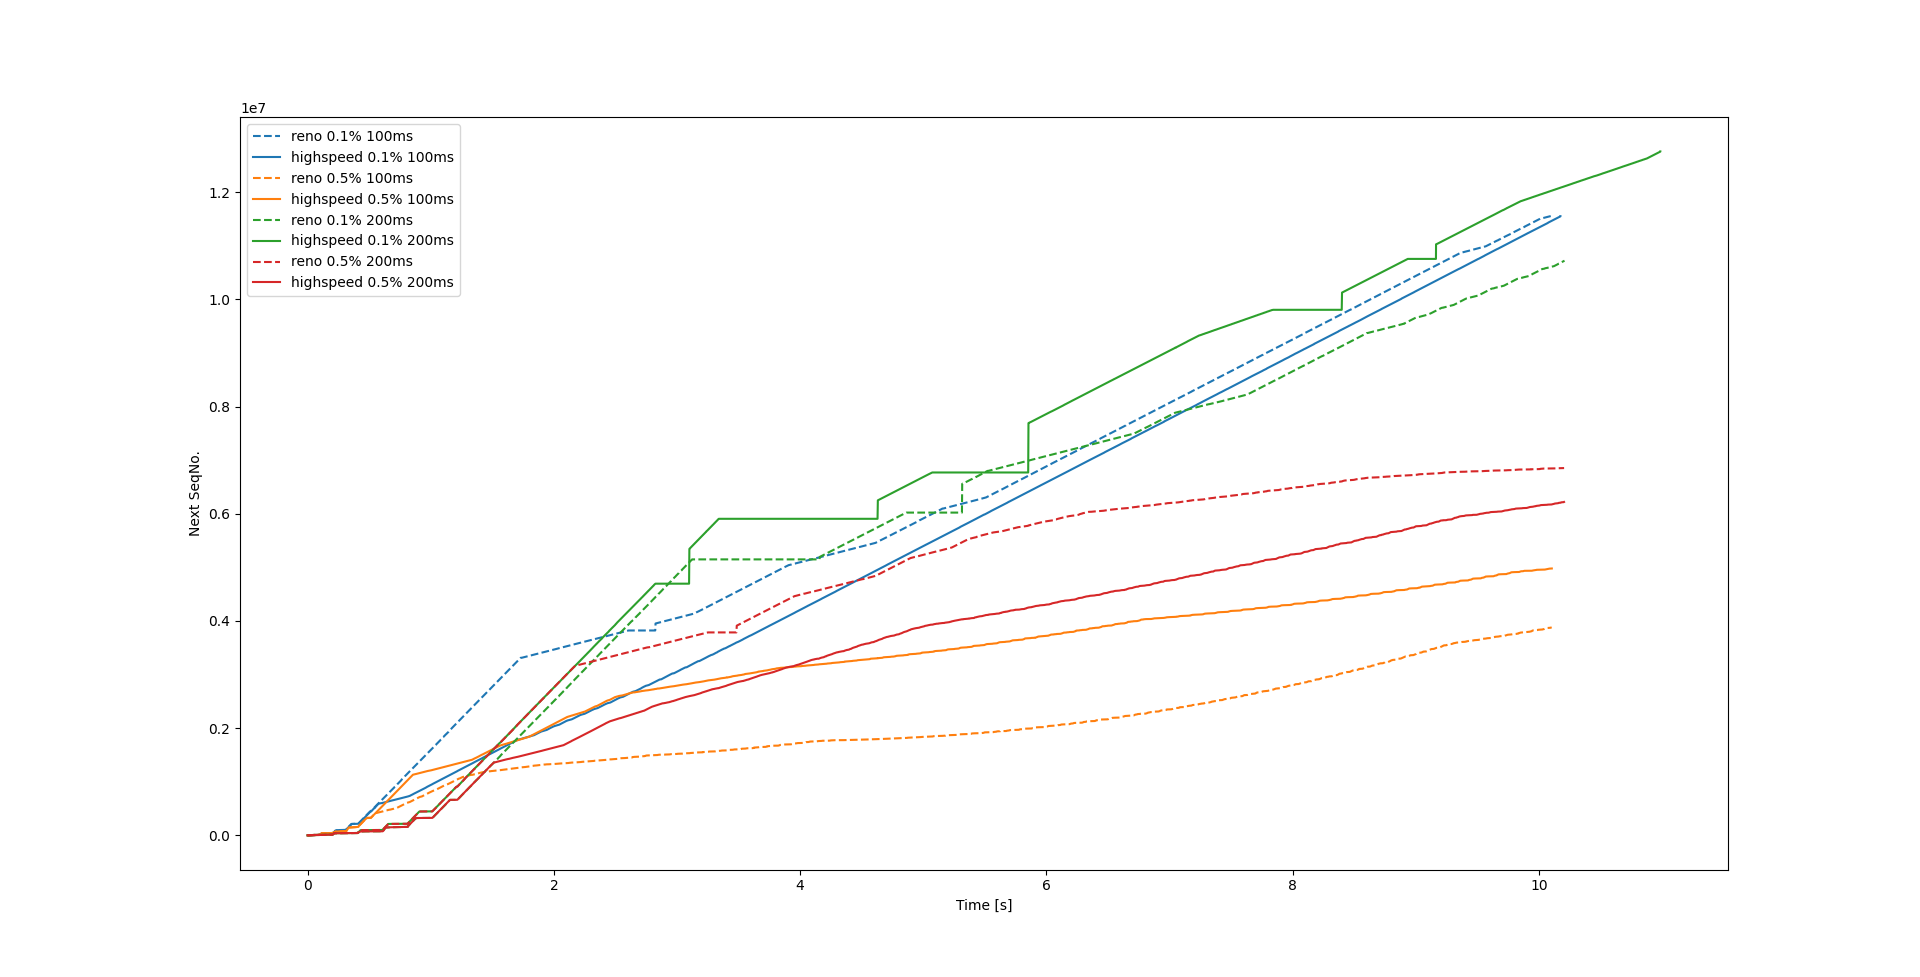
\includegraphics[width=0.75\linewidth]{reno-vs-highspeed-seqno.png}
    \caption{Reno vs Highspeed TCP}
    \label{fig:reno-vs-highpseed}
\end{figure}

\section{DCTCP}
\texttt{Data Center TCP} (\textbf{DCTCP}) congestion control is an an algorithm developed to sustain the needs of large data centers. In general, the traffic in a data center is composed of both long and short flows, that require respectively high throughputs and low latencies; moreover, data centers can often experience sudden bursts, for which many servers address their traffic to the same server at the same time. Considering these aspects, the switches used in data centers need to search for the right trade off between short queues for short flows and long queues for bursts and long flows. \textbf{RFC3168} proposes the \texttt{Explicit Congestion Notification} (\textbf{ECN}) from switches to detect the presence of congestions, but not the extent; in case of not severe congestion, the TCP congestion window is reduced way too much and the throughput of long flows decreases unnecessarily.

\textbf{DCTCP} enhances the \textbf{ECN} approach to estimate the number of bytes that encounter congestion, modifying the \textbf{CWND} accordingly. Going more in depth, the \textbf{ECN} approach expects a specific flag (\textbf{CE}) in the \texttt{IP header} to be set when a packet reaches a switch and the queue in greater than a congestion threshold; then the receiver keeps setting the Explicit Congestion Notification Echo flag (\textbf{ECE}) until a packet with the \texttt{Congestion Window Reduced} (\textbf{CWR}) flag is set; the problem here is that, in \textbf{DCTCP}, it is necessary to have more detailed information from the sender about the congestion, as mentioned before. To achieve so, \textbf{DCTCP} adopts a new \textbf{TCP} state variable to keep the estimated fraction of bytes sent that encountered congestion, called \textbf{DCTCP.Alpha} and initialized to 1; this variable gets updated according to a specific algorithm and the sender will use it to update the \textbf{CWND} as follows:
\[
CWND = CWND * \left(1 - \frac{\text{DCTCP.Alpha}}{2}\right)
\]
It can be observed that, unless the estimated fraction of bytes sent that encountered congestion remains equal to 1, the \textbf{CWND} will not be halved, but it will be reduced by a smaller amount, as the algorithm proposed to achieve. Taking a look at the captures of the experiments conducted with different losses and different delays (figure~\ref{fig:dctcp_delays}), it can be noticed that, when the loss increases, the congestion window gets scaled back in a way that attempts to limit the reduction; of course, it is not easy to predict how the sender is going to update the \textbf{DCTCP.Alpha} parameter, as many details are up to the implementation.
\begin{figure}[h]
    \centering
    \begin{subfigure}{0.45\textwidth}
        \centering
        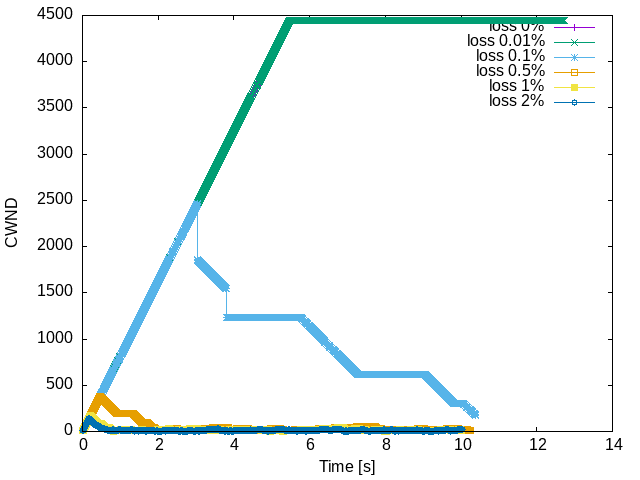
\includegraphics[width=0.8\linewidth]{dctcp_10ms.png}
        \caption{DCTCP 10ms delay}
    \end{subfigure}
    \begin{subfigure}{0.45\textwidth}
        \centering
        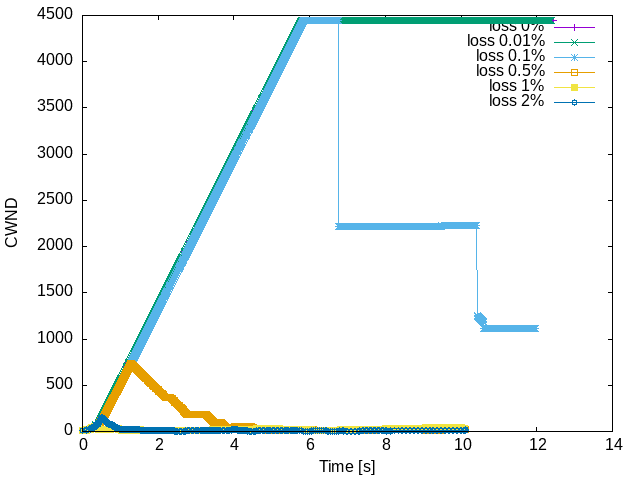
\includegraphics[width=0.8\textwidth]{dctcp_100ms.png}
        \caption{DCTCP 100ms delay}
    \end{subfigure}
    \caption{DCTCP: 10ms vs 100ms delay}
    \label{fig:dctcp_delays}
\end{figure}


\section{Vegas}
\textbf{Vegas TCP} is a delay-based \texttt{Congestion Control} algorithm, which means that, during the connection, also the \texttt{RTT} is taken into consideration when updating the \texttt{CWND}. In \textbf{Reno}, we know that a re-transmission can only happen after three duplicate \texttt{ACK}s are received by the sender, while \textbf{Vegas} takes a different approach: it saves for each segment a \texttt{timestamp} and, after receiving a duplicated \texttt{ACK}, it will check if the difference between the \texttt{timestamp} and the current \texttt{CPU time} is greater than the \texttt{timeout}; if it is, it will re-send the segment. If \textbf{Vegas} receives an unacknowledged \texttt{ACK} that is the first or second after the re-transmission, it will check again if difference between the \texttt{timestamp} of the last packet it sent and the current \texttt{CPU time} is greater than the \texttt{timeout}; if it is, it will re-send the segment in  in case a loss happend (it is to be recalled that \textbf{Reno} would have had to wait 3 duplicated \texttt{ACK}s). \textbf{Vegas} also has a different approach during the \texttt{congestion avoidance} phase, as, after two round trip delays, the\texttt{CWND} is calculated as follows:
\[
(CWND_{\text{current}} - CWND_{\text{previous}}) \cdot (RTT_{\text{current}} - RTT_{\text{previous}})
\]
If this value is positive, the \texttt{CWND} gets reduced by one-eight, while if it is negative or zero (either the \texttt{CWND} was just reduced or we are faster or equal than the previous sample), it is increased by one. This brings \textbf{Vegas} to oscillate around a stable point as we can clearly see in figure~\ref{fig:vegas-10ms}. Although \textbf{Vegas} tries to improve on the \textbf{Reno}'s limitations, it also introduces some new ones: unfortunately, \textbf{Vegas} under-performs when there is a high delay and the reason is that the \texttt{CWND} update is only done after two round trip delays; if there is a high delay, the \texttt{CWND} will not be updated very frequently and we can observe in figure~\ref{fig:vegas-vegas-delay} how this impacts on the overall speed of the connection; in the case of 500ms delay with just a few losses, the \texttt{CWND} is able to gain back some growth.
\begin{figure}[h]
    \centering
    \includegraphics[width=0.45\linewidth]{vegas_10ms.pdf}
    \caption{Vegas 10ms delay}
    \label{fig:vegas-10ms}
\end{figure}
\begin{figure}[h]
    \centering
    \begin{subfigure}{0.45\textwidth}
        \centering
        \includegraphics[width=1\textwidth]{seqno/vegas_10ms.pdf}
        \caption{Vegas 10ms delay}
    \end{subfigure}
    \begin{subfigure}{0.45\textwidth}
        \centering
        \includegraphics[width=1\textwidth]{seqno/vegas_500ms.pdf}
        \caption{Vegas 500ms delay}
    \end{subfigure}
    \caption{Vegas 10ms vs 500ms delay}
    \label{fig:vegas-vegas-delay}
\end{figure}

\section{BBR}
\texttt{Bottleneck Bandwidth and RTT} (\textbf{BBR}) congestion control is an algorithm developed by \texttt{Google}; the aim of this algorithm is to try and maximise the bandwidth of the connection. Unlike \textbf{Reno} or \textbf{Cubic}, which are based on packet losses to make adjustments to the \texttt{CWND}, \textbf{BBR} tries to guess how congested is the network in order to adjust its \texttt{CWND}; as a matter of fact, \textbf{BBR} resides in the kind of \texttt{CCA}s called \textbf{Grey Box} (not\textbf{ White Box} because the information it gets is not the real state of the network, but it is just an internal model which may not reflect reality). \textbf{BBR} has four phases, which alternate between themselves, and they are \textbf{Startup}, \textbf{Drain}, \textbf{Probe Bandwidth}, \textbf{Probe RTT}; the most important ones are \textbf{Probe Bandwidth} and \textbf{Probe RTT}, as during these two phases, for each \textbf{ACK} received, \textbf{BBR} updates its internal values as follows:
\begin{lstlisting}[language=c]
feareach ack
    bottleneck_bandwidth = windowed_max(delivered / elapsed, 10 round trips)
    min_rtt = windowed_min(rtt, 10 seconds)
pacing_rate = pacing_gain * bottleneck_bandwidth
cwnd = max(cwnd_gain * bottleneck_bandwidth * min_rtt, 4)
\end{lstlisting}
We can see how the \texttt{bottleneck\_bandwidth} is calculated as the number of \texttt{packets delivered} divided by the \texttt{elapsed} from the first one, and the packets considered are inside a window which is big at max \texttt{10 round trips}, where each round is a burst that \textbf{BBR} sends. The \texttt{pacing\_rate} is another important parameter which depends on the \texttt{bottleneck\_bandwidth} and on the \texttt{pacing\_gain}, which changes during each of the phases of \textbf{BBR}. Unlike the other \texttt{CCA}s, \textbf{BBR} bases how fast it sends packets on both the \texttt{CWND} and the \texttt{pacing\_rate}; considering what is written on the documentation, the \texttt{CWND} is a countermeasure to stop \textbf{BBR} when it is in the \texttt{Probe Bandwidth} phase, because otherwise it would consume too much bandwidth, filling up the router's queues. About the other two phases, one is \textbf{Startup}, which is the beginning of the connection where the \texttt{CWND} increases like \textbf{Cubic}, until the maximum bandwidth is reached; the other phase is \textbf{Drain}, which has been implemented because \textbf{BBR} is not particularly disposed to share the bandwidth of a shared channel with other \texttt{CCA}s like \textbf{Reno} or \textbf{Cubic}. In order to avoid eating up the whole bandwidth, for a short period of time it decreases on purpose the \texttt{pacing\_gain}, so that, if other loss-based \texttt{CCA}s like Reno need to take their share of the channel, the minimum \texttt{RTT} will increase for \textbf{BBR}, thus decreasing its \texttt{CWND}; after a certain amount in time, given that the event is happening in a stable system, they will come to a situation where they both share equally the channel.

This characteristic of maximising the bandwidth provides \textbf{BBR} with very high resistance to packet losses; we can clearly see in  figure~\ref{fig:bbr-reno-cubic-10ms} and in figure~\ref{fig:bbr-reno-cubic-500ms} how \textbf{BBR} maintains a high throughput on the channel also with a \texttt{2\% packet loss}, while \textbf{Reno} and \textbf{Cubic} reach very low performances. This is even more noticeable when there is high delay, and we can observe that \textbf{Cubic}, with a \texttt{500ms delay} and \texttt{2\% packet loss probability}, exchanges just a total of $10^6$ bytes over 10 seconds on a 10Mb/s channel, while \texttt{BBR} is one degree of magnitude above him in the same conditions.  

\newpage

\section{Appendix}

\subsection{Reno}

\begin{figure}[H]
    \centering
    \begin{subfigure}{0.40\textwidth}
        \centering
        \includegraphics[width=1\textwidth]{reno_10ms_cwnd.pdf}  
        \caption{Reno CWND with 10ms delay}
    \end{subfigure}
    \hfill
    \begin{subfigure}{0.40\textwidth}
        \centering
        \includegraphics[width=1\textwidth]{reno_50ms_cwnd2.pdf}
        \caption{Reno CWND with 50ms delay}
    \end{subfigure}
    \hfill
    \begin{subfigure}{0.40\textwidth}
        \centering
        \includegraphics[width=1\textwidth]{reno_200ms_cwnd.pdf}
        \caption{Reno CWND with 200ms delay}
    \end{subfigure}
    \caption{Reno CWND with different delay comparison}
    \label{fig:reno_cwnd_comparison}
\end{figure}

\begin{figure}[H]
    \centering
    \begin{subfigure}{0.40\textwidth}
        \centering
        \includegraphics[width=1\textwidth]{reno_10ms_rtt.pdf}  
        \caption{Reno RTT with 10ms delay}
    \end{subfigure}
    \hfill
    \begin{subfigure}{0.40\textwidth}
        \centering
        \includegraphics[width=1\textwidth]{reno_50ms_rtt.pdf}
        \caption{Reno RTT with 50ms delay}
    \end{subfigure}
    \hfill
    \begin{subfigure}{0.40\textwidth}
        \centering
        \includegraphics[width=1\textwidth]{reno_200ms_rtt.pdf}
        \caption{Reno RTT with 200ms delay}
    \end{subfigure}
    \caption{Reno RTT with different delay comparison}
    \label{fig:reno_rtt_comparison}
\end{figure}


\pagebreak
\subsection{BBR vs Reno vs Cubic}
\begin{figure}[H]
    \centering
    \begin{subfigure}{0.40\textwidth}
        \centering
        \includegraphics[width=1\textwidth]{bbr_10ms.pdf}
        \caption{BBR with 10ms delay}
    \end{subfigure}
    \begin{subfigure}{0.40\textwidth}
        \centering
        \includegraphics[width=1\textwidth]{reno_10ms_seq.pdf}
        \caption{Reno with 10ms delay}
    \end{subfigure}
    \begin{subfigure}{0.40\textwidth}
        \centering
        \includegraphics[width=1\textwidth]{cubic_10ms.pdf}
        \caption{Cubic with 10ms delay}
    \end{subfigure}
    \caption{BBR vs Reno vs Cubic (10ms delay)}
    \label{fig:bbr-reno-cubic-10ms}
\end{figure}
\begin{figure}
    \centering
    \begin{subfigure}{0.40\textwidth}
        \centering
        \includegraphics[width=1\textwidth]{bbr_500ms.pdf}
        \caption{BBR with 500ms delay}
    \end{subfigure}
    \begin{subfigure}{0.40\textwidth}
        \centering
        \includegraphics[width=1\textwidth]{reno_500ms.pdf}
        \caption{Reno with 500ms delay}
    \end{subfigure}
    \begin{subfigure}{0.40\textwidth}
        \centering
        \includegraphics[width=1\textwidth]{cubic_500ms.pdf}
        \caption{Cubic with 500ms delay}
    \end{subfigure}
    \caption{BBR vs Reno vs Cubic (500ms delay)}
    \label{fig:bbr-reno-cubic-500ms}
\end{figure}

\subsection{Script to generate graphs}
\begin{lstlisting}[language=bash]
#!/bin/bash

if [ -z $1 ]; then
	echo "no parameter"
	exit 1
fi

# insert the tcp_diag module
modprobe tcp_diag
# enable the tcp log tracing
cd /sys/kernel/debug/tracing
echo 1 > events/tcp/tcp_probe/enable
cd -   # get back to the previous folder

#disable tcp metric saving
sysctl net.ipv4.tcp_no_metrics_save=0
#enable/disable SACK
sysctl net.ipv4.tcp_sack=1

INTF=enp2s0

ethtool -K ${INTF} rx off tx off sg off tso off gso off gro off

tc qdisc add dev ${INTF} root netem

algos=("cubic" "reno" "vegas" "dctcp" "highspeed" "bbr")
losses=("0%" "0.01%" "0.1%" "0.5%" "1%" "2%")

function plot_algos {
	mkdir -p afig.cwnd
	mkdir -p afig.sstresh
	mkdir -p afig.seqno
	mkdir -p afig.rtt

	# Plot scripts toghether
	for algo in ${algos[@]}; do
		PLOT_FILES=""
		TITLES=""
		for loss in ${losses[@]}; do
			PLOT_FILES="${PLOT_FILES} ${algo}_${loss}_${1}/data"
			TITLES="${TITLES}'loss $(sed 's/%/\\%/' <<< ${loss})' "
		done
		echo ${PLOT_FILES[*]}

		gnuplot <<EOF
set term pdf
set pointsize 0.3

files='${PLOT_FILES}'
titles="${TITLES}"

set output "afig.cwnd/${algo}_${1}.pdf"
set xlabel "Time [s]"
set ylabel "CWND"
ofs = 0
plot for [i=1:words(files)] word(files, i) using (ofs = (\$0 == 0 ? strcol(1) : ofs), strcol(1) - ofs):5 title word(titles, i) with linespoint

set output "afig.sstresh/${algo}_${1}.pdf"
set xlabel "Time [s]"
set ylabel "SSTRESH"
ofs = 0
plot for [i=1:words(files)] word(files, i) using (ofs = (\$0 == 0 ? strcol(1) : ofs), strcol(1) - ofs):(\$6 < 2000000 ? \$6 : 0) title word(titles, i) with linespoint

set output "afig.seqno/${algo}_${1}.pdf"
set xlabel "Time [s]"
set ylabel "SEQ No."
ofs = 0
seq = 0
plot for [i=1:words(files)] word(files, i) using (ofs = (\$0 == 0 ? strcol(1) : ofs), strcol(1) - ofs):(seq = (\$0 == 0 ? strcol(3) : seq), strcol(3) - seq >= 0 ? strcol(3) - seq : 1/0) title word(titles, i) with linespoint

set output "afig.rtt/${algo}_${1}.pdf"
set xlabel "Time [s]"
set ylabel "RTT [µs]"
ofs = 0
plot for [i=1:words(files)] word(files, i) using (ofs = (\$0 == 0 ? strcol(1) : ofs), strcol(1) - ofs):8 title word(titles, i) with linespoint
EOF
	done
}

mkdir $1
cd $1

#plot_algos $1
#exit 0


ALLOW=""
for algo in ${algos[@]}; do
	modprobe tcp_${algo}
	ALLOW="${ALLOW}${algo} "
	sysctl net.ipv4.tcp_allowed_congestion_control=$(echo ${ALLOW})

	for loss in ${losses[@]}; do
		mkdir ${algo}_${loss}_$1
		cd ${algo}_${loss}_$1

		#set link properties - note that you first have to ADD the netem qdisc before CHANGE it
		#change your params
		tc qdisc change dev ${INTF} root netem loss ${loss} delay $1
		echo tc qdisc change dev ${INTF} root netem loss ${loss} delay $1

		# reset the log file so that we don't get past values
		echo > /sys/kernel/debug/tracing/trace

		# follow the output of trace, the file has capped lenght
		TRACE_FILE=trace
		#tail --follow /sys/kernel/debug/tracing/trace > $TRACE_FILE &
		#TAIL_PID=$!

		SRC_PORT=12345
		SERVER="10.0.3.1"
		iperf3 -c ${SERVER} -C ${algo} --cport ${SRC_PORT}

		#now extract data
		# NOTE: you need to filter the proper TCP connection
		# TBD: may be it's possible to automatize this by parsing iperf3 output?

		cat /sys/kernel/debug/tracing/trace > $TRACE_FILE

		# get time
		cat $TRACE_FILE |grep cwnd| grep $SRC_PORT| tr -s ' '| cut -d ' ' -f 5|cut -d':' -f 1 >time
		#get data len
		cat $TRACE_FILE |grep cwnd| grep $SRC_PORT|cut -d '=' -f6|cut -d ' ' -f 1 >len
		#get SeqNo
		cat $TRACE_FILE |grep cwnd| grep $SRC_PORT|cut -d '=' -f7|cut -d ' ' -f 1 >seqno
		#get ack
		cat $TRACE_FILE |grep cwnd| grep $SRC_PORT|cut -d '=' -f8|cut -d ' ' -f 1 >una
		#get CWND
		cat $TRACE_FILE |grep cwnd| grep $SRC_PORT|cut -d '=' -f9|cut -d ' ' -f 1 >cwnd
		#get ssthresh
		cat $TRACE_FILE |grep cwnd| grep $SRC_PORT|cut -d '=' -f10|cut -d ' ' -f 1 >ssthresh
		#get snd_wnd
		cat $TRACE_FILE |grep cwnd| grep $SRC_PORT|cut -d '=' -f11|cut -d ' ' -f 1 >snd_wnd
		#get rtt
		cat $TRACE_FILE |grep cwnd| grep $SRC_PORT|cut -d '=' -f12|cut -d ' ' -f 1 >rtt
			
		#put everything together	
		paste time len seqno una cwnd ssthresh snd_wnd rtt > data


		#now just quick&dirt plot it - TBD: better prepare a plot.gnu
		gnuplot << EOF
set term png
set xlabel "Time [s]"

#TBD: set proper labels
set ylabel " Len "
set out "len_$algo.png"
plot 'data' using 1:2 title "" with linespoint

set ylabel " SeqNo "
set out "SeqNo_$algo.png" 
plot 'data' using 1:3 title ""  with linespoint

set ylabel " UNA "
set out "una_$algo.png"
plot 'data' using 1:4 title "" with linespoint

set ylabel " CWND "
set out "cwnd_$algo.png"
plot 'data' using 1:5 title "" with linespoint

set ylabel " ssthresh "
set out "ssthresh_$algo.png"
plot 'data' using 1:6 title "" with linespoint

set ylabel " SND WND "
set out "snd_wnd_$algo.png"
plot 'data' using 1:7 title "" with linespoint

set ylabel " rtt "
set out "rtt_$algo.png"
plot 'data' using 1:8 title "" with linespoint

EOF

		cd ..
	done
done

plot_algos $1
\end{lstlisting}


\end{document}